\documentclass[conference]{IEEEtran}
\IEEEoverridecommandlockouts
\usepackage{cite}
\usepackage{amsmath,amssymb}
\usepackage{graphicx}
\usepackage{booktabs}
\usepackage{array}
\usepackage{url}
\Urlmuskip=0mu plus 1mu
\usepackage{placeins}
\usepackage[T1]{fontenc}
\usepackage{newtxtext,newtxmath}
\usepackage{textcomp}
\newcommand{\NTradingDays}{3,161}
\newcommand{\DataStart}{2014-01-01}
\newcommand{\DataEnd}{2026-10-09}
\newcommand{\NEquityRowsM}{5.84}
\newcommand{\NEquityRows}{5,836,673}
\newcommand{\NSymbols}{3,748}
\newcommand{\NFOUnderlyings}{354}
\newcommand{\FOPerDayMin}{134}
\newcommand{\FOPerDayMax}{227}
\newcommand{\NStaleFiles}{92}
\newcommand{\NDelivOverlapDates}{12}
\newcommand{\NDelivOverlapMismatch}{0}
\newcommand{\NFOOverlapDays}{5}
\newcommand{\NAdjust}{1,442}
\newcommand{\NAdjustNSE}{841}
\newcommand{\NAdjustGap}{468}
\newcommand{\NAdjustDemerger}{133}
\newcommand{\NGOneChecks}{57}
\newcommand{\GOneMaxDiff}{0}
\newcommand{\NFeatures}{80}
\newcommand{\NBroadTrain}{2,102}
\newcommand{\NBroadVal}{978}
\newcommand{\NBroadTest}{1,796}
\newcommand{\NBroadTotal}{4,876}
\newcommand{\SuccBroad}{0.262}
\newcommand{\NAllTrain}{5,075}
\newcommand{\NAllVal}{1,979}
\newcommand{\NAllTest}{4,273}
\newcommand{\NAllTotal}{11,327}
\newcommand{\SuccAll}{0.249}
\newcommand{\NStrictTrain}{38}
\newcommand{\NStrictVal}{15}
\newcommand{\NStrictTest}{29}
\newcommand{\NStrictTotal}{82}
\newcommand{\SuccStrict}{0.241}
\newcommand{\TvHOneExp}{27.3}
\newcommand{\TvHOneRest}{26.2}
\newcommand{\TvHOneDiff}{+1.0}
\newcommand{\TvHOneP}{0.513}
\newcommand{\TvHOneQ}{0.94}
\newcommand{\TvHTwoExp}{26.7}
\newcommand{\TvHTwoRest}{26.8}
\newcommand{\TvHTwoP}{0.936}
\newcommand{\TvHThreeExp}{1.03}
\newcommand{\TvHThreeRest}{1.07}
\newcommand{\TvHThreeP}{0.801}
\newcommand{\ValAUCxgb}{0.492}
\newcommand{\ValAUCrf}{0.487}
\newcommand{\ValAUClogit}{0.528}
\newcommand{\ValAUCcomp}{0.506}
\newcommand{\XgbTrees}{14}
\newcommand{\XgbDepth}{2}
\newcommand{\HOneExp}{24.8}
\newcommand{\HOneRest}{24.9}
\newcommand{\HOneDiff}{\ensuremath{-}0.04}
\newcommand{\HOneP}{0.987}
\newcommand{\HOneQ}{0.987}
\newcommand{\HTwoExp}{23.5}
\newcommand{\HTwoRest}{26.3}
\newcommand{\HTwoDiff}{\ensuremath{-}2.81}
\newcommand{\HTwoP}{0.171}
\newcommand{\HTwoQ}{0.286}
\newcommand{\HThreeExp}{1.01}
\newcommand{\HThreeRest}{0.88}
\newcommand{\HThreeP}{0.384}
\newcommand{\HThreeQ}{0.480}
\newcommand{\AUCxgb}{0.460}
\newcommand{\AUCrf}{0.466}
\newcommand{\AUClogit}{0.468}
\newcommand{\AUCcomp}{0.526}
\newcommand{\HFourDiff}{\ensuremath{-}0.066}
\newcommand{\HFourSE}{0.023}
\newcommand{\HFourP}{0.005}
\newcommand{\HFourQ}{0.024}
\newcommand{\TopMLPrec}{22.4}
\newcommand{\TopCompPrec}{31.0}
\newcommand{\TopMLN}{165}
\newcommand{\TopP}{0.108}
\newcommand{\TopSpread}{\ensuremath{-}0.26}
\newcommand{\TopSpreadLo}{\ensuremath{-}1.29}
\newcommand{\TopSpreadHi}{+0.64}
\newcommand{\BrierRaw}{0.250}
\newcommand{\BrierCal}{0.195}
\newcommand{\WFAUC}{0.502}
\newcommand{\WFMonths}{46}
\newcommand{\NPHTwoDiff}{\ensuremath{-}5.65}
\newcommand{\NPHTwoP}{0.026}
\newcommand{\NPHTwoQ}{0.128}
\newcommand{\NPHFourDiff}{\ensuremath{-}0.039}
\newcommand{\NPHFourP}{0.141}
\newcommand{\BHm}{5}
\newcommand{\BaseRateTest}{0.248}
\newcommand{\TTwoDiff}{+0.8}
\newcommand{\TTwoP}{0.586}
\newcommand{\PowRuleN}{144}
\newcommand{\PowRuleDiff}{\ensuremath{-}0.2}
\newcommand{\PowRuleP}{0.978}
\newcommand{\LadBaseN}{159,972}
\newcommand{\LadBase}{26.7}
\newcommand{\LadAll}{24.9}
\newcommand{\LadAllDiff}{\ensuremath{-}1.9}
\newcommand{\LadAllP}{0.005}
\newcommand{\LadBroad}{24.8}
\newcommand{\LadComp}{41.4}
\newcommand{\LadCompN}{29}
\newcommand{\CagrAll}{\ensuremath{-}26.8}
\newcommand{\TradesAll}{2,736}
\newcommand{\MaxDDAll}{\ensuremath{-}68.6}
\newcommand{\CagrBroad}{\ensuremath{-}12.6}
\newcommand{\TradesBroad}{1,599}
\newcommand{\MaxDDBroad}{\ensuremath{-}39.2}
\newcommand{\CagrComp}{+6.0}
\newcommand{\TradesComp}{29}
\newcommand{\MaxDDComp}{\ensuremath{-}1.0}
\newcommand{\CagrML}{+4.3}
\newcommand{\TradesML}{157}
\newcommand{\MaxDDML}{\ensuremath{-}2.3}
\newcommand{\CagrNifty}{+9.7}
\newcommand{\SPAp}{0.77}
\newcommand{\CashRate}{6}
\newcommand{\SharpeComp}{\ensuremath{-}0.01}
\newcommand{\SharpeML}{\ensuremath{-}0.85}
\newcommand{\MaxPositions}{20}
\newcommand{\RCp}{0.89}
\newcommand{\DSRtrials}{89}
\newcommand{\TrialsBefore}{67}
\newcommand{\TrialsTestRun}{22}
\newcommand{\TrialsThroughPSix}{89}
\newcommand{\PreregCommit}{15103f1}
\newcommand{\PreregTime}{08:54}
\newcommand{\LockHead}{ea49def}
\newcommand{\LockStart}{09:23}
\newcommand{\LockCommit}{359bcc7}
\newcommand{\LockCommitTime}{09:30}
\newcommand{\TostHOneLo}{\ensuremath{-}3.7}
\newcommand{\TostHOneHi}{+3.6}
\newcommand{\TostHOneP}{0.19}
\newcommand{\TostHTwoLo}{\ensuremath{-}6.2}
\newcommand{\TostHTwoHi}{+0.6}
\newcommand{\TostHTwoP}{0.65}
\newcommand{\TostNPHOneLo}{\ensuremath{-}1.9}
\newcommand{\TostNPHOneHi}{+7.2}
\newcommand{\TostNPHOneP}{0.59}
\newcommand{\TostNPHTwoLo}{\ensuremath{-}9.8}
\newcommand{\TostNPHTwoHi}{\ensuremath{-}1.5}
\newcommand{\TostNPHTwoP}{0.93}
\newcommand{\MDEHOne}{6.26}
\newcommand{\MDEHTwo}{5.71}
\newcommand{\ExpN}{47}
\newcommand{\ExpRemoved}{331}
\newcommand{\ExpDiff}{\ensuremath{-}1.4}
\newcommand{\ExpP}{0.572}
\newcommand{\ExpPMin}{0.516}
\newcommand{\PSIpcr}{0.55}
\newcommand{\PSIclient}{0.31}
\newcommand{\PSInModerate}{7}
\newcommand{\PSInLarge}{2}
\newcommand{\BrierConstVal}{0.188}
\newcommand{\BrierConstTest}{0.187}
\newcommand{\IncompleteBroad}{4}
\newcommand{\GapEvents}{165}
\newcommand{\GapTrades}{157}
\newcommand{\GapSlotsFull}{8}
\newcommand{\RoundTrip}{0.58}
\newcommand{\RTLarge}{0.45}
\newcommand{\RTSmall}{0.75}
\newcommand{\AvgWin}{+4.74}
\newcommand{\AvgLoss}{\ensuremath{-}1.85}
\newcommand{\WinLossSpread}{6.59}
\newcommand{\BreakEven}{8.8}
\newcommand{\BEHOneDiff}{\ensuremath{-}0.0}
\newcommand{\BEHOneLo}{\ensuremath{-}4.4}
\newcommand{\BEHOneHi}{+4.3}
\newcommand{\BEHOneBLo}{\ensuremath{-}5.3}
\newcommand{\BEHOneBHi}{+4.7}
\newcommand{\BEHOneN}{1265}
\newcommand{\BEHTwoDiff}{\ensuremath{-}2.8}
\newcommand{\BEHTwoLo}{\ensuremath{-}6.8}
\newcommand{\BEHTwoHi}{+1.2}
\newcommand{\BEHTwoBLo}{\ensuremath{-}8.3}
\newcommand{\BEHTwoBHi}{+2.1}
\newcommand{\BEHTwoN}{924}
\newcommand{\BENPHOneDiff}{+2.6}
\newcommand{\BENPHOneLo}{\ensuremath{-}2.8}
\newcommand{\BENPHOneHi}{+8.1}
\newcommand{\BENPHOneBLo}{\ensuremath{-}2.8}
\newcommand{\BENPHOneBHi}{+7.9}
\newcommand{\BENPHOneN}{899}
\newcommand{\BENPHTwoDiff}{\ensuremath{-}5.6}
\newcommand{\BENPHTwoLo}{\ensuremath{-}10.6}
\newcommand{\BENPHTwoHi}{\ensuremath{-}0.7}
\newcommand{\BENPHTwoBLo}{\ensuremath{-}12.3}
\newcommand{\BENPHTwoBHi}{+0.7}
\newcommand{\BENPHTwoN}{617}
\newcommand{\BEMLDiff}{\ensuremath{-}2.7}
\newcommand{\BEMLLo}{\ensuremath{-}9.4}
\newcommand{\BEMLHi}{+4.1}
\newcommand{\BEMLBLo}{\ensuremath{-}13.8}
\newcommand{\BEMLBHi}{+7.3}
\newcommand{\BEMLN}{165}
\newcommand{\BECompTopDiff}{+7.0}
\newcommand{\BECompTopLo}{+0.6}
\newcommand{\BECompTopHi}{+13.4}
\newcommand{\BECompTopBLo}{+0.8}
\newcommand{\BECompTopBHi}{+15.0}
\newcommand{\BECompTopN}{226}
\newcommand{\BECompRuleDiff}{+16.8}
\newcommand{\BECompRuleLo}{\ensuremath{-}1.2}
\newcommand{\BECompRuleHi}{+34.9}
\newcommand{\BECompRuleBLo}{\ensuremath{-}10.0}
\newcommand{\BECompRuleBHi}{+46.3}
\newcommand{\BECompRuleN}{29}
\newcommand{\BEnBelow}{3}
\newcommand{\SpecOneN}{54}
\newcommand{\SpecOnePred}{89}
\newcommand{\SpecOneSig}{15}
\newcommand{\SpecOneSigPct}{28}
\newcommand{\SpecOneOpp}{0}
\newcommand{\SpecOneBH}{3}
\newcommand{\SpecOneMedian}{+2.36}
\newcommand{\SpecOneMax}{5.05}
\newcommand{\SpecOneCIAbove}{4}
\newcommand{\SpecOneFrozen}{\ensuremath{-}0.04}
\newcommand{\SpecOneRank}{49}
\newcommand{\SpecTwoN}{18}
\newcommand{\SpecTwoPred}{94}
\newcommand{\SpecTwoSig}{3}
\newcommand{\SpecTwoSigPct}{17}
\newcommand{\SpecTwoOpp}{0}
\newcommand{\SpecTwoBH}{0}
\newcommand{\SpecTwoMedian}{\ensuremath{-}2.24}
\newcommand{\SpecTwoMax}{4.44}
\newcommand{\SpecTwoCIAbove}{0}
\newcommand{\SpecTwoFrozen}{\ensuremath{-}2.81}
\newcommand{\SpecTwoRank}{6}
\newcommand{\BFOneUni}{17.88}
\newcommand{\BFNPOneUni}{9.31}
\newcommand{\BFOneSkep}{2.27}
\newcommand{\BFNPOneSkep}{1.27}
\newcommand{\BFOneLogDef}{8.41}
\newcommand{\BFNPOneLogDef}{4.49}
\newcommand{\BFOneLogSkep}{2.32}
\newcommand{\BFNPOneLogSkep}{1.43}
\newcommand{\BFTwoUni}{7.65}
\newcommand{\BFNPTwoUni}{1.31}
\newcommand{\BFTwoSkep}{1.05}
\newcommand{\BFNPTwoSkep}{0.23}
\newcommand{\BFTwoLogDef}{3.63}
\newcommand{\BFNPTwoLogDef}{0.67}
\newcommand{\BFTwoLogSkep}{1.13}
\newcommand{\BFNPTwoLogSkep}{0.30}
\newcommand{\EOneBOne}{+0.008}
\newcommand{\EOneBOneLo}{\ensuremath{-}0.237}
\newcommand{\EOneBOneHi}{+0.254}
\newcommand{\EOneBOneP}{0.946}
\newcommand{\EOneBTwo}{\ensuremath{-}0.225}
\newcommand{\EOneBTwoLo}{\ensuremath{-}0.592}
\newcommand{\EOneBTwoHi}{+0.142}
\newcommand{\EOneBTwoP}{0.229}
\newcommand{\EOneBThree}{+0.246}
\newcommand{\EOneBThreeLo}{\ensuremath{-}0.130}
\newcommand{\EOneBThreeHi}{+0.622}
\newcommand{\EOneBThreeP}{0.200}
\newcommand{\ETwoBOne}{\ensuremath{-}0.129}
\newcommand{\ETwoBOneLo}{\ensuremath{-}0.361}
\newcommand{\ETwoBOneHi}{+0.102}
\newcommand{\ETwoBOneP}{0.273}
\newcommand{\ETwoBTwo}{+0.185}
\newcommand{\ETwoBTwoLo}{+0.006}
\newcommand{\ETwoBTwoHi}{+0.364}
\newcommand{\ETwoBTwoP}{0.043}
\newcommand{\ETwoBThree}{\ensuremath{-}0.186}
\newcommand{\ETwoBThreeLo}{\ensuremath{-}0.435}
\newcommand{\ETwoBThreeHi}{+0.063}
\newcommand{\ETwoBThreeP}{0.142}
\newcommand{\EMonthMatches}{exactly}
\newcommand{\FYears}{12}
\newcommand{\FYearsSig}{0}
\newcommand{\FFirstYear}{2015}
\newcommand{\FLastYear}{2026}
\newcommand{\GTieShareLoss}{0.12}
\newcommand{\GTieExplained}{0.1}
\newcommand{\GDayOneBO}{15.0}
\newcommand{\GDayOneNB}{10.3}
\newcommand{\GRangeBO}{1.07}
\newcommand{\GRangeNB}{0.95}
\newcommand{\GGapBO}{0.11}
\newcommand{\GGapNB}{0.05}
\newcommand{\GATRBO}{2.55}
\newcommand{\GATRNB}{2.68}
\newcommand{\GAgree}{100.0}
\newcommand{\placeboDraws}{1,000}
\newcommand{\placeboActual}{\ensuremath{-}0.04}
\newcommand{\placeboMean}{+1.65}
\newcommand{\placeboSD}{1.97}
\newcommand{\placeboP}{0.795}
\newcommand{\placeboPct}{20}
\newcommand{\PSevenActual}{+1.05}
\newcommand{\PSevenDraws}{20}
\newcommand{\PSevenGE}{0}

\begin{document}

\title{Do Delivery and Futures-Positioning Footprints Predict Breakout Success? A Pre-Registered Test on Survivorship-Free NSE Data}

\author{
\IEEEauthorblockN{Anonymous Authors}
}

\maketitle

\begin{abstract}
Indian traders read two free daily footprints as signs of informed activity in a stock: the delivery
percentage, the share of traded quantity settled into investors' accounts, and changes in futures positioning.
We ask whether they predict which price breakouts succeed. We rebuild a survivorship-free,
corporate-action-adjusted panel of official National Stock Exchange of India (NSE) files (\DataStart{} to
\DataEnd, \NSymbols{} symbols), label breakouts with a triple barrier (two average true ranges up, one down,
10 days) and test four hypotheses committed to version control before any confirmatory analysis; the test set
(January 2023 to \DataEnd) was evaluated once. None is supported. Delivery expansion changes test-set success
by \HOneDiff{} percentage points (pp) ($p=\HOneP$); rising price with falling open interest points the
predicted way (\HTwoDiff{} pp) but fails false-discovery control ($q=\HTwoQ$); a gradient-boosted model
ranks breakouts worse than a fixed-weight composite (area under the curve \AUCxgb{} vs.\ \AUCcomp). The
design could detect effects of about \MDEHOne{} pp, so smaller effects cannot be ruled out. In post-hoc
analyses on the full test set, the 95\% confidence intervals for the delivery and open-interest effects stay
within the \BreakEven{} pp change in success rate needed to pay one round trip of Indian trading costs, and
after costs no strategy beats the Nifty~500 index.
\end{abstract}

\begin{IEEEkeywords}
backtest overfitting, breakout, delivery percentage, multiple testing, National Stock Exchange of India, open
interest, pre-registration
\end{IEEEkeywords}

\section{Introduction}
Theories of informed trading predict that better-informed traders leave traces in prices and order flow
\cite{kyle1985,glosten1985}, and measures of informed trading and ``flow toxicity'' have been built on
intraday data \cite{easley1996,easley2012}. These theories are motivation only: we do \emph{not} measure
order-flow toxicity and use no intraday data. Our setting is the free end-of-day data of the National Stock
Exchange of India (NSE), in which traders read two footprints of informed activity: the delivery percentage,
and futures positioning, i.e.\ a stock's own open interest (OI) and the market-wide positions NSE reports for
foreign institutional investors (FIIs), domestic institutional investors (DIIs), proprietary desks and
clients. A common belief is that a breakout carried by high delivery and supportive positioning is ``real''.

Because published signals are often chosen after many specifications are tried \cite{harvey2016,bailey2014pseudo},
we built the study so that a negative answer would be credible \cite{nosek2018}, and pre-registered four
hypotheses on BROAD compression breakouts (defined in Section~\ref{sec:method}). \textbf{H1}: breakouts whose
base shows delivery expansion succeed more often. \textbf{H2}: breakouts where price rises while the stock's
futures OI falls succeed less often. \textbf{H3}: breakouts during FII net selling and DII net buying show a
better gain-to-loss ratio. \textbf{H4}: a gradient-boosted tree model (XGBoost \cite{chen2016}) on the same
features beats a fixed-weight composite in the area under the receiver operating characteristic curve (AUC)
and in top-decile precision.

The contributions are four: (i) IMPI, a pipeline that rebuilds a survivorship-free, point-in-time (PIT)
NSE panel, including pre-2019 delivery data that NSE no longer serves in its current format; (ii) a
pre-registered design with a test set opened once and a disclosed timeline; (iii) a confirmatory null
reported with its minimum detectable effect and a cost-based reading of what effect sizes matter; (iv) clearly
separated post-hoc robustness analyses showing how far the null extends and where it does not.

\section{Related Work}
\emph{Informed-flow theory.} Kyle's insider trades gradually so prices absorb information \cite{kyle1985}; in
Glosten--Milgrom the spread prices adverse selection \cite{glosten1985}; the probability of informed trading
(PIN) and its volume-synchronized variant (VPIN) estimate informed trading from trade imbalances
\cite{easley1996,easley2012}. All need trade-level data; we borrow only the intuition that informed activity
may leave a daily footprint.
\emph{Institutional flow in India.} FIIs sold Indian stocks quickly after an unexpected tax-policy shock and
chased past returns \cite{thapa2026}. Firm-level daily FII flows are not public, so participant positioning
can act here only as a market regime. We found no peer-reviewed test of NSE delivery or futures positioning
as a predictor of breakout success.
\emph{Machine learning (ML) for stock prediction.} Nonlinear models are reported to beat linear baselines
\cite{fieberg2023,azevedo2023,lu2025,farimani2024,gonzaleznunez2025}, though rarely on unseen firms
\cite{lu2024}; Shapley additive explanations (SHAP) for tree ensembles \cite{lundberg2020} are now common in
financial ML \cite{cerneviciene2024,martins2024,yeo2025}. We test XGBoost against a simple rule.
\emph{Multiple testing and backtest overfitting.} Significance thresholds must rise with the number of tests
\cite{harvey2016}; the deflated Sharpe ratio (DSR) corrects for trials and non-normality \cite{bailey2014dsr}.
We use the Benjamini--Hochberg (BH) procedure \cite{benjamini1995}, Hansen's test for superior predictive
ability (SPA) \cite{hansen2005} and White's Reality Check \cite{white2000}, and log every trial.

\section{Data and Method}\label{sec:method}
\begin{figure*}[t]
\centering
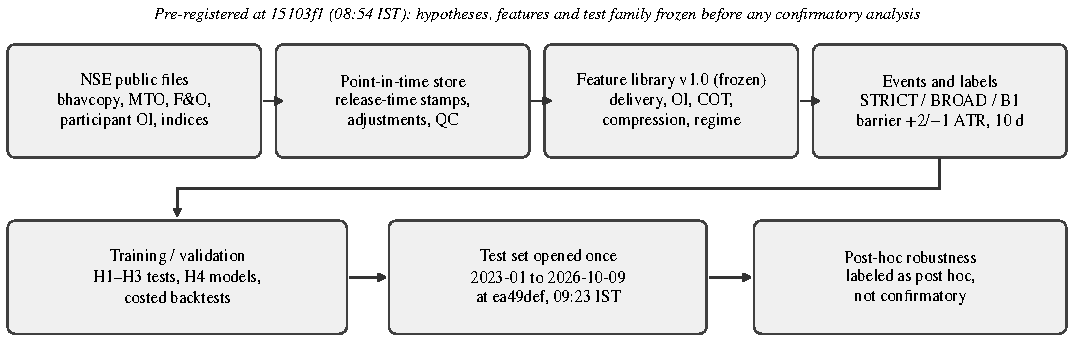
\includegraphics[width=\textwidth]{figs/fig1_pipeline.pdf}
\caption{The IMPI pipeline. Every stage reads only data published by the decision time.}
\label{fig:pipeline}
\end{figure*}

\emph{Data} (Fig.~\ref{fig:pipeline}; Table~\ref{tab:dataset}). Public NSE end-of-day files give
\NTradingDays{} trading days and \NEquityRowsM{} million daily equity rows for \NSymbols{} symbols, delisted
stocks included. Eligibility for the futures and options (F\&O) segment is taken PIT (\NFOUnderlyings{}
underlyings, \FOPerDayMin--\FOPerDayMax{} per day). Pre-2019 delivery is rebuilt from the legacy equity file
and the security-wise delivery-position file (MTO), matching the modern file with \NDelivOverlapMismatch{}
mismatches on \NDelivOverlapDates{} overlap dates; \NAdjust{} split, bonus and demerger adjustments are applied
to prices, volumes and OI, and files are checked by automated quality control (QC).

\emph{Universe and look-ahead.} Tier~1 holds F\&O stocks on the day, excluding ban-list days, announced
results windows, prices below Rs~20 and short histories. Splits are training (June 2015--2020), validation
(2021--2022) and test (January 2023 to \DataEnd), purging events whose label crosses a boundary. Features for
day $T$ use only data released by 23:59 Indian Standard Time (IST) on $T$; trades enter at the $T+1$ open.
Recomputing features on \NGOneChecks{} truncated copies changed no past value.

\emph{Events and label.} STRICT events are an algorithmic volatility contraction pattern (VCP)
\cite{minervini2013}; BROAD events are closes above the prior 20-day high after compression (Bollinger-width
percentile below 30 on 5 of the previous 10 days); B1 is every 20-day-high close (Table~\ref{tab:events}).
With entry $E$ at the $T+1$ open and $A$ the 14-day average true range (ATR), $y=1$ if $E+2A$ is hit before
$E-A$ within 10 days and $y=0$ otherwise \cite{lopezdeprado2018}; a day touching both barriers is a loss, and
\IncompleteBroad{} BROAD events with incomplete windows are excluded.

\begin{table}[t]
\centering
\caption{Dataset summary (official NSE files)}
\label{tab:dataset}
\footnotesize
\setlength{\tabcolsep}{4pt}
\begin{tabular}{@{}>{\raggedright\arraybackslash}p{3.7cm}>{\raggedright\arraybackslash}p{4.4cm}@{}}
\toprule
\textbf{Item} & \textbf{Value} \\
\midrule
Period & 2014-01-01 to 2026-10-09 \\
Trading days & 3,161 \\
Daily equity rows & 5,836,673 \\
Symbols (incl.\ delisted) & 3,748 \\
Futures and options (F\&O) underlyings & 354 over time; 134--227 per day \\
Delivery rebuild vs.\ modern file & 0 mismatches on 12 overlap dates \\
F\&O old vs.\ new file format & 0 mismatches on 5 overlap days \\
Stale files rejected & 92 \\
Duplicate symbol-date rows & 0 \\
Delivery coverage (worst year) & 99.33\% \\
Corporate-action adjustments & 1,442 \\
\bottomrule
\end{tabular}
\end{table}
\begin{table}[t]
\centering
\caption{Tier-1 eligible events by split (frozen before registration)}
\label{tab:events}
\footnotesize
\setlength{\tabcolsep}{4pt}
\begin{tabular}{@{}lrrrrr@{}}
\toprule
\textbf{Event set} & \textbf{Train} & \textbf{Val.} & \textbf{Test} & \textbf{Purged} & \textbf{Success} \\
\midrule
STRICT (VCP) & 38 & 15 & 29 & 1 & 0.241 \\
BROAD & 2,102 & 978 & 1,796 & 131 & 0.262 \\
B1 (20-day highs) & 5,075 & 1,979 & 4,273 & 282 & 0.249 \\
\bottomrule
\end{tabular}
\par\smallskip\parbox{0.98\linewidth}{\scriptsize\raggedright Purged = label window crosses a split boundary or is incomplete. Success = share with label$_{10}=1$ (all splits).}
\end{table}

\emph{Tests and models.} The \NFeatures{} frozen features cover delivery, volume, illiquidity, compression,
VCP, stock OI, commitments-of-traders (COT) style participant positioning in index and stock futures, basis,
put--call ratio and regime. H1 and H2 compare success rates (two-proportion $z$-test, calendar-month block
bootstrap); H3 compares the gain-to-loss ratio, mean favorable over mean adverse excursion. The logistic model
\begin{equation}
\operatorname{logit}\Pr(y=1)=\beta_0+\beta_1 D+\beta_2 P+\beta_3 (D\times P)+\gamma^{\top}x,
\label{eq:logit}
\end{equation}
where $D$ is the exposure and $P$ a second factor (H1: positioning alignment; H2: delivery $z$-score),
estimates the interaction $\beta_3$, with turnover, volatility, liquidity and sector controls $x$. The
pre-registered family has eight tests (H1--H3 on STRICT and BROAD, H4-AUC, H4-top-decile) under BH at
$q=0.10$; no $p$-value is computed for a group with fewer than 30 events. XGBoost, a random forest and logistic
regression are tuned by purged, embargoed 5-fold cross-validation, calibrated isotonically on validation data
and compared with the composite by DeLong's test \cite{delong1988}. Backtests trade Rs~10~lakh in at most
\MaxPositions{} equal-weight positions with full Indian delivery costs and 5--20 basis points of slippage per
side, against the Nifty~500.

\section{Pre-Registration and Integrity}\label{sec:prereg}
Hypotheses, events, test family and decision rules were committed in \texttt{\PreregCommit} at \PreregTime{}
IST on 10 October 2026, with the frozen features (Table~\ref{tab:timeline}). \emph{Lock:} the single test run
started at \LockStart{} IST at commit \texttt{\LockHead} (code plus training/validation results) and wrote the
lock file itself, first committed in \texttt{\LockCommit} at \LockCommitTime. \emph{Trials:} of
\TrialsThroughPSix{} results-log rows up to the test evaluation, \TrialsBefore{} preceded the test run and
\TrialsTestRun{} were written by it; the DSR used all \DSRtrials{} (conservative). \emph{Disclosure:} data
download, corporate-action fixes and QC used the full period; for its power calculation the pre-registration
lists each split's event counts and overall success rate, test included, but no result split by any
hypothesis exposure. Our pilot study had explored July 2025 to October 2026, so confirmatory results are also
reported without that window.

\begin{table}[t]
\centering
\caption{Pre-registration timeline, 10 Oct 2026 (IST, from git and run logs)}
\label{tab:timeline}
\footnotesize
\setlength{\tabcolsep}{4pt}
\begin{tabular}{@{}ll>{\raggedright\arraybackslash}p{5.9cm}@{}}
\toprule
\textbf{Commit} & \textbf{Time} & \textbf{Event} \\
\midrule
\texttt{355cbe0} & 02:16 & Pipeline scaffolding: ingest, PIT store, features, labels \\
\texttt{86ddfd7} & 08:21 & Corporate-action adjustment fixes (full data) \\
\texttt{b5829b2} & 08:40 & Ban-list publication-time fix (look-ahead check) \\
-- & 08:53 & Feature freeze written (features, events, labels) \\
\texttt{15103f1} & 08:54 & Pre-registration (H1--H4, rules, power) and feature freeze \\
-- & 08:54 & First training/validation analysis rows logged \\
\texttt{ea49def} & 09:23 & Training/validation results and model freeze \\
-- & 09:23 & Test run starts: test set opened; lock written (HEAD = ea49def) \\
\texttt{359bcc7} & 09:30 & One-time test evaluation and lock file \\
\texttt{1fc97ae} & 12:01 & First post-hoc work (v2 models, live mode) \\
\bottomrule
\end{tabular}
\par\smallskip\parbox{0.98\linewidth}{\scriptsize\raggedright 67 of the 89 results-log rows up to the test evaluation were written before the test run; the other 22 are the test run's own rows. The lock file was first committed in 359bcc7. Data download, adjustment fixes and QC (before the pre-registration) used the full period. The pre-registration itself lists test-set event counts and the overall test success rate (power table), but no result split by any hypothesis exposure.}
\end{table}

\section{Results}
\subsection{Exploratory (Training and Validation)}
On training and validation data, BROAD breakouts with delivery expansion succeeded \TvHOneExp\% of the time
against \TvHOneRest\% without it, a difference of \TvHOneDiff{} percentage points (pp; $p=\TvHOneP$); H2 rates were \TvHTwoExp\% and
\TvHTwoRest\% ($p=\TvHTwoP$); H3 ratios \TvHThreeExp{} and \TvHThreeRest{} ($p=\TvHThreeP$). Validation AUC
was \ValAUCxgb{} for XGBoost, which stopped early at \XgbTrees{} trees of depth \XgbDepth, \ValAUCrf{} for the
random forest, \ValAUClogit{} for the logistic model and \ValAUCcomp{} for the composite.

\subsection{Confirmatory (Test Set, Run Once, Pre-Registered)}
All STRICT groups have fewer than 30 events per arm, so their $p$-values are withheld and BH runs over
$m=\BHm$ finite $p$-values (Table~\ref{tab:confirm}). No hypothesis is supported. \textbf{H1:} \HOneExp\% vs.\
\HOneRest\% (\HOneDiff{} pp, $p=\HOneP$). \textbf{H2:} \HTwoExp\% vs.\ \HTwoRest\% (\HTwoDiff{} pp,
$q=\HTwoQ$); without the pilot window \NPHTwoDiff{} pp ($p=\NPHTwoP$, $q=\NPHTwoQ$). \textbf{H3:}
\HThreeExp{} vs.\ \HThreeRest{} ($p=\HThreeP$). \textbf{H4:} XGBoost AUC \AUCxgb{} vs.\ \AUCcomp{} for the
composite (difference \HFourDiff, DeLong $p=\HFourP$, $q=\HFourQ$), the only rejection, in the wrong
direction; forest \AUCrf, logit \AUClogit, walk-forward (\WFMonths{} refits) \WFAUC; top-decile precision
\TopMLPrec\% vs.\ \TopCompPrec\% ($p=\TopP$).

The model leaned on market-wide positioning features whose distribution shifted: post hoc, the population
stability index (PSI) is \PSIpcr{} for the put--call ratio and \PSIclient{} for client index-futures
positioning, above the usual 0.25 threshold. Calibration lowered the Brier score \cite{brier1950} from
\BrierRaw{} to \BrierCal, still worse than a constant forecast at the validation base rate (\BrierConstVal).

\emph{Power.} The design has 80\% power at $\alpha=0.05$ for \MDEHOne{} pp (H1) and \MDEHTwo{} pp (H2);
smaller effects cannot be ruled out. Equivalence within $\pm$2 pp is not established (post-hoc two one-sided
tests (TOST) \cite{lakens2017}: 90\% intervals [\TostHOneLo, \TostHOneHi] pp, $p=\TostHOneP$, and
[\TostHTwoLo, \TostHTwoHi] pp, $p=\TostHTwoP$).

\begin{table}[t]
\centering
\caption{Pre-registered confirmatory family on the test set (BH, $q=0.10$, $m=5$)}
\label{tab:confirm}
\footnotesize
\setlength{\tabcolsep}{4pt}
\begin{tabular}{llrrrcr}
\toprule
\textbf{Test} & \textbf{Set} & $n$ & \textbf{Diff.} & $p$ & \textbf{Rank} & $q$ \\
\midrule
\multicolumn{7}{l}{\textit{Full test set (2023-01-01 to 2026-10-09)}} \\
H1 & STRICT & 29 & +12.99 & n$<$30 (0.484) & -- & -- \\
H2 & STRICT & 28 & +11.28 & n$<$30 (0.468) & -- & -- \\
H3 & STRICT & 29 & \ensuremath{-}0.077 & n$<$30 (0.942) & -- & -- \\
H1 & BROAD & 1,796 & \ensuremath{-}0.04 & 0.987 & 5 & 0.987 \\
H2 & BROAD & 1,776 & \ensuremath{-}2.81 & 0.171 & 3 & 0.286 \\
H3 & BROAD & 1,769 & +0.124 & 0.384 & 4 & 0.480 \\
H4 auc & BROAD & 1,796 & \ensuremath{-}0.066 & 0.005 & 1 & 0.024 \\
H4 top decile & BROAD & 1,796 & \ensuremath{-}8.55 & 0.108 & 2 & 0.270 \\
\midrule
\multicolumn{7}{l}{\textit{Without pilot window (before 2025-07-28)}} \\
H1 & STRICT & 23 & +13.33 & n$<$30 (0.567) & -- & -- \\
H2 & STRICT & 22 & +13.33 & n$<$30 (0.484) & -- & -- \\
H3 & STRICT & 23 & +0.622 & n$<$30 (0.478) & -- & -- \\
H1 & BROAD & 1,236 & +2.62 & 0.352 & 4 & 0.440 \\
H2 & BROAD & 1,221 & \ensuremath{-}5.65 & 0.026 & 1 & 0.128 \\
H3 & BROAD & 1,213 & \ensuremath{-}0.083 & 0.759 & 5 & 0.759 \\
H4 auc & BROAD & 1,236 & \ensuremath{-}0.039 & 0.141 & 2 & 0.351 \\
H4 top decile & BROAD & 1,236 & \ensuremath{-}9.37 & 0.258 & 3 & 0.430 \\
\bottomrule
\end{tabular}
\par\smallskip\parbox{0.98\linewidth}{\scriptsize\raggedright PRE-REGISTERED. Diff.\ in pp for H1, H2 and H4-top-decile; H3 = difference in gain-to-loss asymmetry ratio; H4-AUC = AUC difference XGBoost $-$ composite. STRICT tests have fewer than 30 events per arm, so the pre-registered guard withholds their $p$ (unguarded value in brackets, not used); BH therefore runs over $m=5$ finite $p$-values. The only rejection (H4-AUC) is in the wrong direction: XGBoost ranks worse than the composite. No hypothesis is supported.}
\end{table}

\subsection{Backtests (Pre-Registered)}
After costs (Table~\ref{tab:backtests}) all breakouts returned \CagrAll\% a year and BROAD \CagrBroad\%. The
composite (\TradesComp{} trades) and the ML top decile (\TradesML{} trades)\footnote{Fewer trades than events
because signals arriving while all \MaxPositions{} position slots are full are skipped (\GapSlotsFull{} ML
top-decile signals).} returned \CagrComp\% and \CagrML\%, below the Nifty~500's \CagrNifty\% and close to the
\CashRate\% a year that idle cash earns in the backtest; their Sharpe ratios of \SharpeComp{} and
\SharpeML{} show no return above cash. SPA ($p=\SPAp$) and the Reality Check ($p=\RCp$) find no strategy
beating the benchmark. Breakouts succeed less often than all eligible stock-days (\LadAll\% vs.\ \LadBase\%,
Fig.~\ref{fig:ladder}).

\begin{table}[t]
\centering
\caption{Costed test-set backtests (2023-01 to 2026-10)}
\label{tab:backtests}
\footnotesize
\setlength{\tabcolsep}{4pt}
\begin{tabular}{@{}lrrrr@{}}
\toprule
\textbf{Strategy} & \textbf{Trades} & \textbf{CAGR\%} & \textbf{Sharpe} & \textbf{MaxDD\%} \\
\midrule
All breakouts & 2,736 & \ensuremath{-}26.8 & \ensuremath{-}4.02 & \ensuremath{-}68.6 \\
BROAD & 1,599 & \ensuremath{-}12.6 & \ensuremath{-}3.25 & \ensuremath{-}39.2 \\
Composite $\geq$ 1 & 29 & +6.0 & \ensuremath{-}0.01 & \ensuremath{-}1.0 \\
ML top decile & 157 & +4.3 & \ensuremath{-}0.85 & \ensuremath{-}2.3 \\
\midrule
Nifty 500 & -- & +9.7 & 0.32 & \ensuremath{-}18.8 \\
\bottomrule
\end{tabular}
\par\smallskip\parbox{0.98\linewidth}{\scriptsize\raggedright Pre-registered (test set, run once). CAGR = compound annual growth rate; MaxDD = maximum drawdown. Full Indian costs; at most 20 positions. SPA $p$ = 0.77, Reality Check $p$ = 0.89; deflated Sharpe ratio $\approx 0$ for all. All variants are available from the authors on request.}
\end{table}

\begin{figure}[t]
\centering
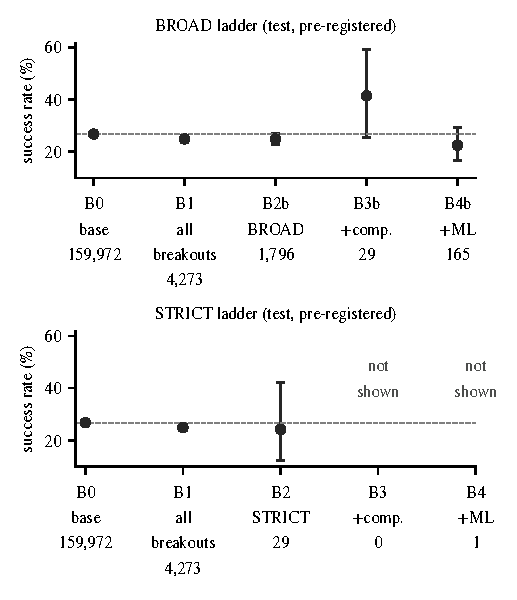
\includegraphics[width=\columnwidth]{figs/fig_ladder.pdf}
\caption{Pre-registered benchmark ladder in the test period: ten-day success rate with Wilson 95\% intervals;
the dashed line is the base rate over all eligible stock-days. Rungs with fewer than two events are labeled,
not plotted.}
\label{fig:ladder}
\end{figure}

\subsection{Post-Hoc Analyses}
\emph{All analyses in this subsection were designed after the test set was opened.}

\textbf{Cost break-even.} A round trip costs \RoundTrip\% on average (\RTLarge--\RTSmall\%); successes return
\AvgWin\% and failures \AvgLoss\% gross, so a success-rate change $d$ pays one round trip only if
$d\ge\BreakEven$ pp. The 95\% intervals for H1 (\BEHOneLo{} to \BEHOneHi; month-block \BEHOneBLo{} to
\BEHOneBHi), H1 without pilot (\BENPHOneLo{} to \BENPHOneHi) and H2 (\BEHTwoLo{} to \BEHTwoHi) lie inside
$\pm$\BreakEven{} pp. H2 without the pilot window (\NPHTwoDiff{} pp; \BENPHTwoLo{} to \BENPHTwoHi) reaches
the break-even. The composite top decile beats other BROAD events by \BECompTopDiff{} pp (\BECompTopLo{} to
\BECompTopHi), excluding zero but not the break-even.

\textbf{Placebo.} Shuffling delivery across stocks within each day \placeboDraws{} times gives a mean placebo
H1 effect of \placeboMean{} pp (SD \placeboSD), not zero: delivery expansion is a $z$-score against each
stock's own trailing year, and a within-day shuffle keeps the market-wide delivery level, so the placebo
exposure retains a time-varying market component. It is therefore not a clean null. The actual
\placeboActual{} pp sits at its \placeboPct{}th percentile (one-sided $p=\placeboP$; Fig.~\ref{fig:placebo}):
no stock-specific delivery information beyond that component. The training/validation H1 effect of
\PSevenActual{} pp, larger than all \PSevenDraws{} placebo draws there, is not reproduced.

\begin{figure}[t]
\centering
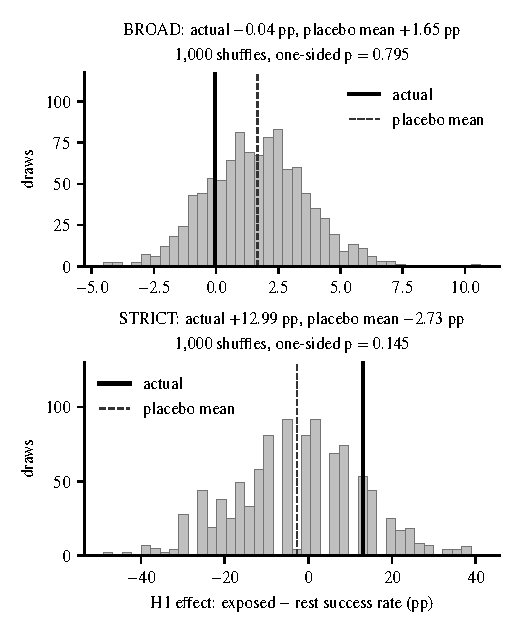
\includegraphics[width=\columnwidth]{figs/fig_placebo_hist.pdf}
\caption{Post-hoc placebo on the test set: H1 effect under within-day shuffles of delivery across stocks,
with the actual effect marked. The shuffle distribution is not centered at zero (see text).}
\label{fig:placebo}
\end{figure}

\textbf{Specification curve.} Varying barrier, horizon, delivery threshold and event set
(Fig.~\ref{fig:spec}) \cite{simonsohn2020}, \SpecOnePred\% of \SpecOneN{} H1 specifications point the
predicted way, \SpecOneSig{} are significant at 5\% (\SpecOneOpp{} opposite) and \SpecOneBH{} survive BH; the
median is \SpecOneMedian{} pp and the maximum \SpecOneMax{} pp, below the break-even. The pre-registered
specification (\SpecOneFrozen{} pp) ranks \SpecOneRank{} of \SpecOneN: stricter thresholds and wider barriers
give larger effects. For H2, \SpecTwoSig{} of \SpecTwoN{} are significant, \SpecTwoBH{} survive, median
\SpecTwoMedian{} pp; the frozen specification ranks \SpecTwoRank. The specifications overlap and are not
independent.

\begin{figure*}[t]
\centering
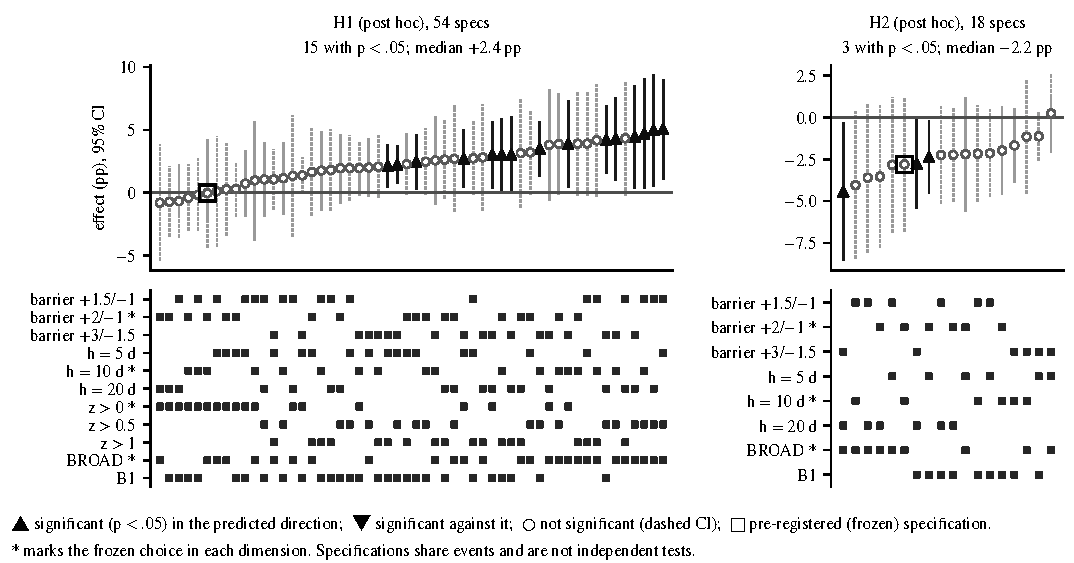
\includegraphics[width=\textwidth]{figs/fig_spec_curve.pdf}
\caption{Post-hoc specification curve on the test set: effect and 95\% confidence interval per specification
(top) and its choices (bottom); the square marks the pre-registered specification.}
\label{fig:spec}
\end{figure*}

\textbf{Bayes factors.} BF$_{01}$ for H1 is \BFOneUni{} (uniform priors \cite{kass1995}) and \BFOneLogDef{}
(unit-normal log-odds prior \cite{gronau2021}) but only \BFOneSkep--\BFOneLogSkep{} under skeptical priors;
for H2 \BFTwoUni, \BFTwoLogDef{} and \BFTwoSkep--\BFTwoLogSkep. Without the pilot window, H2 under the
skeptical beta prior gives \BFNPTwoSkep{}, i.e.\ moderate evidence \emph{for} a difference. The null is
strongly favored only under wide priors \cite{leewagenmakers2013}.

\textbf{Cluster-robust model.} With two-way date $\times$ stock clustering \cite{cameron2011}, the test-set
interaction in \eqref{eq:logit} is $\beta_3=\EOneBThree$ [\EOneBThreeLo, \EOneBThreeHi] ($p=\EOneBThreeP$)
for H1 and \ETwoBThree{} ($p=\ETwoBThreeP$) for H2. The H2 model's delivery term, \ETwoBTwo{}
($p=\ETwoBTwoP$), is a single post-hoc coefficient with no multiplicity adjustment.

\textbf{Other checks.} Dropping the 5 sessions before each of \ExpN{} F\&O expiries leaves H1 at
\ExpDiff{} pp ($p=\ExpP$); \FYearsSig{} of \FYears{} yearly H1 estimates are significant. Same-day barrier
ties are \GTieShareLoss\% of breakout losses, but breakouts are stopped out on day one more often
(\GDayOneBO\% vs.\ \GDayOneNB\%) on wider next-day ranges.

\section{Discussion and Limitations}
The pre-registered answer is no: delivery expansion, OI divergence and the FII/DII regime do not detectably
change breakout success, and boosted trees do worse than a fixed composite, consistent with drift in
market-wide positioning features. The null is informative about large effects only: the detectable effect is
about \MDEHOne{} pp, $\pm$2 pp equivalence is not established, and Bayes factors favor the null strongly only
under wide priors. Post hoc, the full-test intervals sit below the \BreakEven{} pp cost break-even. One subset
does not fit: without the pilot window, H2 is \NPHTwoDiff{} pp ($p=\NPHTwoP$, $q=\NPHTwoQ$), its 95\% interval
reaches the break-even, and the skeptical-prior BF$_{01}$ of \BFNPTwoSkep{} is moderate evidence for H2. As a
post-hoc look at a subset that fails false-discovery control, it is a lead, not a finding. In the
specification curve the pre-registered H1 specification is among the weakest; stricter delivery thresholds or
wider barriers give post-hoc effects of a few pp, perhaps information about move size rather than direction,
that mostly fail multiple-testing control and stay below break-even.

\emph{Limitations.} Participant positions are market-wide only, futures positions may be hedges, and the
``Client'' class mixes retail and wealthy accounts. STRICT events are too rare for inference. The sample spans
T+1 settlement (2023) and F\&O reforms (2024--2025). Registration followed full-period data preparation and
disclosed test-set counts and base rates, and our pilot overlapped the test period. The post-hoc analyses are
many and were chosen after the result was known.

\section{Conclusion and Future Work}
With a survivorship-free NSE panel, hypotheses fixed in advance and a test set opened once, we find no support
for the belief that delivery and futures-positioning footprints predict breakout success, and no strategy that
beats the Nifty~500 after costs. Smaller effects remain possible, but on the full test set they are below what
Indian costs require. Four leads need their own pre-registered tests on post-October-2026 data: (1) whether
FIIs follow price in stock futures; (2) whether FII index-futures positioning precedes index returns; (3)
whether stricter delivery thresholds predict breakout move size; (4) whether price-up/OI-down divergence (H2)
predicts breakout failure, as the post-hoc subset without the pilot window suggests. We also plan a
market-level regime-transition model using participant positioning to forecast volatility regimes,
pre-registered and evaluated only on post-October-2026 data. Nothing here is investment advice.

\section*{Data and Code Availability}
Inputs are public NSE end-of-day files, re-downloaded by the pipeline. Code, configuration, locked and
post-hoc results, the generators of every table, figure and number, and SHA-256 checksums of the locked files
are available from the authors on request.

\section*{Acknowledgment}
The authors used Claude (Anthropic) via Claude Code to write and debug portions of the IMPI pipeline code,
run the post-hoc audit and robustness scripts, generate the \LaTeX{} tables and figures from the logged
results, and draft and edit text in all sections. The research question, hypotheses, pre-registration, data
sources and all interpretive decisions were made by the authors, who reviewed and verified all AI-generated
code, text and figures and take full responsibility for the content of this paper.

\FloatBarrier
\begin{thebibliography}{10}
\providecommand{\url}[1]{#1}
\csname url@samestyle\endcsname
\providecommand{\newblock}{\relax}
\providecommand{\bibinfo}[2]{#2}
\providecommand{\BIBentrySTDinterwordspacing}{\spaceskip=0pt\relax}
\providecommand{\BIBentryALTinterwordstretchfactor}{4}
\providecommand{\BIBentryALTinterwordspacing}{\spaceskip=\fontdimen2\font plus
\BIBentryALTinterwordstretchfactor\fontdimen3\font minus
  \fontdimen4\font\relax}
\providecommand{\BIBforeignlanguage}[2]{{%
\expandafter\ifx\csname l@#1\endcsname\relax
\typeout{** WARNING: IEEEtran.bst: No hyphenation pattern has been}%
\typeout{** loaded for the language `#1'. Using the pattern for}%
\typeout{** the default language instead.}%
\else
\language=\csname l@#1\endcsname
\fi
#2}}
\providecommand{\BIBdecl}{\relax}
\BIBdecl

\bibitem{kyle1985}
A.~S. Kyle, ``Continuous auctions and insider trading,'' \emph{Econometrica},
  vol.~53, no.~6, pp. 1315--1335, 1985, doi: \url{10.2307/1913210}.

\bibitem{glosten1985}
L.~R. Glosten and P.~R. Milgrom, ``Bid, ask and transaction prices in a
  specialist market with heterogeneously informed traders,'' \emph{J. Financial
  Econ.}, vol.~14, no.~1, pp. 71--100, 1985, doi:
  \url{10.1016/0304-405X(85)90044-3}.

\bibitem{easley1996}
D.~Easley, N.~M. Kiefer, M.~O'Hara, and J.~B. Paperman, ``Liquidity,
  information, and infrequently traded stocks,'' \emph{J. Finance}, vol.~51,
  no.~4, pp. 1405--1436, 1996, doi: \url{10.1111/j.1540-6261.1996.tb04074.x}.

\bibitem{easley2012}
D.~Easley, M.~M. L{\'o}pez~de Prado, and M.~O'Hara, ``Flow toxicity and
  liquidity in a high-frequency world,'' \emph{Rev. Financial Stud.}, vol.~25,
  no.~5, pp. 1457--1493, 2012, doi: \url{10.1093/rfs/hhs053}.

\bibitem{harvey2016}
C.~R. Harvey, Y.~Liu, and H.~Zhu, ``{\ldots}and the cross-section of expected
  returns,'' \emph{Rev. Financial Stud.}, vol.~29, no.~1, pp. 5--68, 2016, doi:
  \url{10.1093/rfs/hhv059}.

\bibitem{bailey2014pseudo}
D.~H. Bailey, J.~M. Borwein, M.~L{\'o}pez~de Prado, and Q.~J. Zhu,
  ``Pseudo-mathematics and financial charlatanism: The effects of backtest
  overfitting on out-of-sample performance,'' \emph{Notices Amer. Math. Soc.},
  vol.~61, no.~5, pp. 458--471, 2014, doi: \url{10.1090/noti1105}.

\bibitem{nosek2018}
B.~A. Nosek, C.~R. Ebersole, A.~C. DeHaven, and D.~T. Mellor, ``The
  preregistration revolution,'' \emph{Proc. Nat. Acad. Sci. USA}, vol. 115,
  no.~11, pp. 2600--2606, 2018, doi: \url{10.1073/pnas.1708274114}.

\bibitem{chen2016}
T.~Chen and C.~Guestrin, ``{XGBoost}: A scalable tree boosting system,'' in
  \emph{Proc. 22nd ACM SIGKDD Int. Conf. Knowl. Discov. Data Mining}, 2016, pp.
  785--794, doi: \url{10.1145/2939672.2939785}.

\bibitem{thapa2026}
C.~Thapa, B.~Neupane, C.~Shrestha, and N.~P. Bhattarai, ``Policy information
  uncertainty and foreign institutional investors trading behavior: Evidence
  from {India},'' \emph{Rev. Quant. Finance Account.}, vol.~67, pp. 45--79,
  2026, doi: \url{10.1007/s11156-025-01448-8}.

\bibitem{fieberg2023}
C.~Fieberg, D.~Metko, T.~Poddig, and T.~Loy, ``Machine learning techniques for
  cross-sectional equity returns' prediction,'' \emph{OR Spectr.}, vol.~45,
  no.~1, pp. 289--323, 2023, doi: \url{10.1007/s00291-022-00693-w}.

\bibitem{azevedo2023}
V.~Azevedo and C.~Hoegner, ``Enhancing stock market anomalies with machine
  learning,'' \emph{Rev. Quant. Finance Account.}, vol.~60, no.~1, pp.
  195--230, 2023, doi: \url{10.1007/s11156-022-01099-z}.

\bibitem{lu2025}
X.~Lu, J.~Poon, and M.~Khushi, ``Leveraging {BiLSTM-GAT} for enhanced stock
  market prediction: A dual-graph approach to portfolio optimization,''
  \emph{Appl. Intell.}, vol.~55, no.~7, p. 601, 2025, doi:
  \url{10.1007/s10489-025-06462-w}.

\bibitem{farimani2024}
S.~A. Farimani, M.~V. Jahan, and A.~M. Fard, ``An adaptive multimodal learning
  model for financial market price prediction,'' \emph{IEEE Access}, vol.~12,
  pp. 121\,846--121\,863, 2024, doi: \url{10.1109/ACCESS.2024.3441029}.

\bibitem{gonzaleznunez2025}
E.~Gonz{\'a}lez-N{\'u}{\~n}ez, L.~A. Trejo, and M.~Kampouridis, ``Expanding a
  machine learning class towards its application to the stock market
  forecast,'' \emph{Appl. Intell.}, vol.~55, no.~1, p.~21, 2025, doi:
  \url{10.1007/s10489-024-06018-4}.

\bibitem{lu2024}
X.~Lu, J.~Poon, and M.~Khushi, ``Bridging the gap between machine and human in
  stock prediction: Addressing heterogeneity in stock market,'' \emph{IEEE
  Access}, vol.~12, pp. 186\,171--186\,185, 2024, doi:
  \url{10.1109/ACCESS.2024.3511613}.

\bibitem{lundberg2020}
S.~M. Lundberg, G.~Erion, H.~Chen, A.~DeGrave, J.~M. Prutkin, B.~Nair, R.~Katz,
  J.~Himmelfarb, N.~Bansal, and S.-I. Lee, ``From local explanations to global
  understanding with explainable {AI} for trees,'' \emph{Nature Mach. Intell.},
  vol.~2, no.~1, pp. 56--67, 2020, doi: \url{10.1038/s42256-019-0138-9}.

\bibitem{cerneviciene2024}
J.~{\v{C}}ernevi{\v{c}}ien{\.{e}} and A.~Kaba{\v{s}}inskas, ``Explainable
  artificial intelligence ({XAI}) in finance: A systematic literature review,''
  \emph{Artif. Intell. Rev.}, vol.~57, p. 216, 2024, doi:
  \url{10.1007/s10462-024-10854-8}.

\bibitem{martins2024}
T.~Martins, A.~M. de~Almeida, E.~Cardoso, and L.~Nunes, ``Explainable
  artificial intelligence ({XAI}): A systematic literature review on taxonomies
  and applications in finance,'' \emph{IEEE Access}, vol.~12, pp. 618--629,
  2024, doi: \url{10.1109/ACCESS.2023.3347028}.

\bibitem{yeo2025}
W.~J. Yeo, W.~Van Der~Heever, R.~Mao, E.~Cambria, R.~Satapathy, and
  G.~Mengaldo, ``A comprehensive review on financial explainable {AI},''
  \emph{Artif. Intell. Rev.}, vol.~58, no.~6, p. 189, 2025, doi:
  \url{10.1007/s10462-024-11077-7}.

\bibitem{bailey2014dsr}
D.~H. Bailey and M.~L{\'o}pez~de Prado, ``The deflated {Sharpe} ratio:
  Correcting for selection bias, backtest overfitting, and non-normality,''
  \emph{J. Portfolio Manage.}, vol.~40, no.~5, pp. 94--107, 2014, doi:
  \url{10.3905/jpm.2014.40.5.094}.

\bibitem{benjamini1995}
Y.~Benjamini and Y.~Hochberg, ``Controlling the false discovery rate: A
  practical and powerful approach to multiple testing,'' \emph{J. Roy. Statist.
  Soc. Ser. B (Methodol.)}, vol.~57, no.~1, pp. 289--300, 1995, doi:
  \url{10.1111/j.2517-6161.1995.tb02031.x}.

\bibitem{hansen2005}
P.~R. Hansen, ``A test for superior predictive ability,'' \emph{J. Bus. Econ.
  Statist.}, vol.~23, no.~4, pp. 365--380, 2005, doi:
  \url{10.1198/073500105000000063}.

\bibitem{white2000}
H.~White, ``A reality check for data snooping,'' \emph{Econometrica}, vol.~68,
  no.~5, pp. 1097--1126, 2000, doi: \url{10.1111/1468-0262.00152}.

\bibitem{minervini2013}
M.~Minervini, \emph{Trade Like a Stock Market Wizard}.\hskip 1em plus 0.5em
  minus 0.4em\relax New York: McGraw-Hill, 2013.

\bibitem{lopezdeprado2018}
M.~L{\'o}pez~de Prado, \emph{Advances in Financial Machine Learning}.\hskip 1em
  plus 0.5em minus 0.4em\relax Hoboken, NJ: Wiley, 2018.

\bibitem{delong1988}
E.~R. DeLong, D.~M. DeLong, and D.~L. Clarke-Pearson, ``Comparing the areas
  under two or more correlated receiver operating characteristic curves: A
  nonparametric approach,'' \emph{Biometrics}, vol.~44, no.~3, pp. 837--845,
  1988, doi: \url{10.2307/2531595}.

\bibitem{brier1950}
G.~W. Brier, ``Verification of forecasts expressed in terms of probability,''
  \emph{Monthly Weather Rev.}, vol.~78, no.~1, pp. 1--3, 1950, doi:
  \url{10.1175/1520-0493(1950)078<0001:VOFEIT>2.0.CO;2}.

\bibitem{lakens2017}
D.~Lakens, ``Equivalence tests: A practical primer for $t$ tests, correlations,
  and meta-analyses,'' \emph{Social Psychol. Personality Sci.}, vol.~8, no.~4,
  pp. 355--362, 2017, doi: \url{10.1177/1948550617697177}.

\bibitem{simonsohn2020}
U.~Simonsohn, J.~P. Simmons, and L.~D. Nelson, ``Specification curve
  analysis,'' \emph{Nature Human Behav.}, vol.~4, no.~11, pp. 1208--1214, 2020,
  doi: \url{10.1038/s41562-020-0912-z}.

\bibitem{kass1995}
R.~E. Kass and A.~E. Raftery, ``Bayes factors,'' \emph{J. Amer. Statist.
  Assoc.}, vol.~90, no. 430, pp. 773--795, 1995, doi:
  \url{10.1080/01621459.1995.10476572}.

\bibitem{gronau2021}
Q.~F. Gronau, A.~Raj K.~N., and E.-J. Wagenmakers, ``Informed {Bayesian}
  inference for the {A/B} test,'' \emph{J. Statist. Softw.}, vol. 100, no.~17,
  2021, doi: \url{10.18637/jss.v100.i17}.

\bibitem{leewagenmakers2013}
M.~D. Lee and E.-J. Wagenmakers, \emph{Bayesian Cognitive Modeling: A Practical
  Course}.\hskip 1em plus 0.5em minus 0.4em\relax Cambridge: Cambridge
  University Press, 2013.

\bibitem{cameron2011}
A.~C. Cameron, J.~B. Gelbach, and D.~L. Miller, ``Robust inference with
  multiway clustering,'' \emph{J. Bus. Econ. Statist.}, vol.~29, no.~2, pp.
  238--249, 2011, doi: \url{10.1198/jbes.2010.07136}.

\end{thebibliography}

\end{document}